\section{Der Heiratssatz}\label{kapitel:Heiratssatz}
Lösungen von Kombinatorikaufgaben sind häufig lang und konfus, denn hier ist es viel schwieriger (als zum Beispiel\ in Geometrie), eure Ideen in klare Formeln und Worte zu fassen. Dementsprechend häufig sind unvollständige Lösungen und Punktabzüge. An dieser Stelle kann häufig der \emph{Heiratssatz} aushelfen und aus einem \enquote{Wurschtelargument} eine saubere, wasserfeste Lösung machen, bzw.\ euch überhaupt erst auf eine vernünftige Lösung führen.

Bevor wir den Satz formulieren und beweisen können, müssen wir ein wenig Terminologie einführen. Erinnert euch (siehe das Kapitel ~\emph{Graphentheorie} im Heft für Klasse~9), dass ein \emph{bipartiter Graph} ein Graph $G=(V,E)$ ist, dessen Knotenmenge $V=A\cup B$ sich in zwei disjunkte Teilmengen $A$ und $B$ zerlegen lässt, sodass Kanten nur zwischen $A$ und $B$ verlaufen, aber nicht innerhalb von $A$ oder $B$. Ein \emph{Matching} in einem bipartiten Graphen $G=(A\cup B, E)$ ist eine Teilmenge $M\subseteq E$ von Kanten, sodass $M$ für jeden Knoten von $G$ höchstens eine ausgehende Kante enthält. Die folgende Abbildung zeigt einen bipartiten Graphen $G$ sowie zwei mögliche Matchings $M_1$ und $M_2$ in $G$.

\begin{figure}[ht]
	\centering
	\begin{tabularx}{\textwidth}{X c X c X c X}
		& 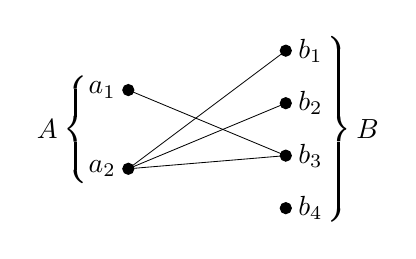
\begin{tikzpicture}
			\draw[fill=black] (0,0) circle (2pt) node[left=0.1em] {$a_1$};
			\draw[fill=black] (0,-1) circle (2pt) node[left=0.1em] {$a_2$};
			\draw[fill=black] (2,0.5) circle (2pt) node[right=0.1em] {$b_1$};
			\draw[fill=black] (2,-0.167) circle (2pt) node[right=0.1em] {$b_2$};
			\draw[fill=black] (2,-0.833) circle (2pt) node[right=0.1em] {$b_3$};
			\draw[fill=black] (2,-1.5) circle (2pt) node[right=0.1em] {$b_4$};
			\draw[line width=0.3] (0,0) -- (2,-0.833);
			\draw[line width=0.3] (0,-1) -- (2,-0.167);
			\draw[line width=0.3] (0,-1) -- (2,0.5);
			\draw[line width=0.3] (0,-1) -- (2,-0.833);
			\path (0,0) -- (0,-1) node[pos=0.5, left=2.2em] {$A$} node[pos=0.5, below=1.2em, sloped] {$\underbrace{\hspace{1.35cm}}$};
			\path (2,-1.5) -- (2,0.5) node[pos=0.5,right=2.2em] {$B$} node[pos=0.5, below=1.2em, sloped] {$\underbrace{\hspace{2.35cm}}$};
		\end{tikzpicture} & & 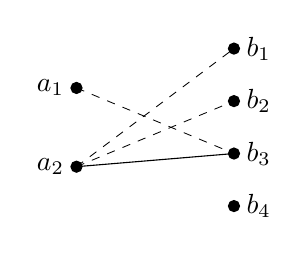
\begin{tikzpicture}
			\draw[fill=black] (0,0) circle (2pt) node[left=0.1em] {$a_1$};
			\draw[fill=black] (0,-1) circle (2pt) node[left=0.1em] {$a_2$};
			\draw[fill=black] (2,0.5) circle (2pt) node[right=0.1em] {$b_1$};
			\draw[fill=black] (2,-0.167) circle (2pt) node[right=0.1em] {$b_2$};
			\draw[fill=black] (2,-0.833) circle (2pt) node[right=0.1em] {$b_3$};
			\draw[fill=black] (2,-1.5) circle (2pt) node[right=0.1em] {$b_4$};
			\draw[line width=0.3,dashed] (0,0) -- (2,-0.833);
			\draw[line width=0.3,dashed] (0,-1) -- (2,-0.167);
			\draw[line width=0.3,dashed] (0,-1) -- (2,0.5);
			\draw (0,-1) -- (2,-0.833);
		\end{tikzpicture} & & 
		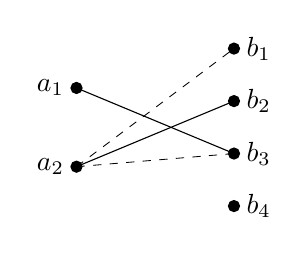
\begin{tikzpicture}
			\draw[fill=black] (5.5,0) circle (2pt) node[left=0.1em] {$a_1$};
			\draw[fill=black] (5.5,-1) circle (2pt) node[left=0.1em] {$a_2$};
			\draw[fill=black] (7.5,0.5) circle (2pt) node[right=0.1em] {$b_1$};
			\draw[fill=black] (7.5,-0.167) circle (2pt) node[right=0.1em] {$b_2$};
			\draw[fill=black] (7.5,-0.833) circle (2pt) node[right=0.1em] {$b_3$};
			\draw[fill=black] (7.5,-1.5) circle (2pt) node[right=0.1em] {$b_4$};
			\draw (5.5,0) -- (7.5,-0.833);
			\draw (5.5,-1) -- (7.5,-0.167);
			\draw[line width=0.3,dashed] (5.5,-1) -- (7.5,0.5);
			\draw[line width=0.3,dashed] (5.5,-1) -- (7.5,-0.833);
		\end{tikzpicture} & \\
		& bipartiter Graph & & Matching $M_1$ & & Matching $M_2$ &
	\end{tabularx} 
\end{figure}

Die Matchings $M_1$ und $M_2$ sind zugleich \emph{inklusionsmaximale Matchings}: Würden wir nämlich noch irgendeine weitere Kante zu $M_1$ oder $M_2$ hinzufügen, dann würden mindestens zwei Kanten der Matchings von einem der Knoten $b_3$ oder $a_2$ ausgehen und wir hätten kein Matching mehr.

Der \emph{Heiratssatz}
geht nun der Frage nach, für welche bipartiten Graphen $G=(A\cup B,E)$ ein Matching $M$ existiert, das alle Knoten von $A$ überdeckt. Für den obigen Graphen ist dies offenbar der Fall, denn $M_2$ ist genau ein solches Matching. Gleichzeitig zeigt das Beispiel, dass \emph{nicht} jedes inklusionsmaximale Matching diese Bedingung erfüllt. Das Problem ist also nicht völlig trivial. Um den Heiratssatz formulieren zu können, müssen wir noch folgende Notation einführen: Für jede Teilmenge $S\subseteq A$ soll $N_G(S)$ die Menge aller Knoten aus $B$ sein, die mit mindestens einem Knoten aus $S$ durch eine Kante verbunden sind. Im obigen Beispiel ist etwa $N(\{a_1\})=\{b_3\}$ und $N(A)=\{b_1,b_2,b_3\}$. Der Heiratssatz besagt nun Folgendes:
\begin{satzmitnamen}[Heiratssatz]
	In einem bipartiten Graphen $G=(A\cup B,E)$ existiert genau dann ein Matching, das alle Knoten aus $A$ überdeckt, wenn für jede Teilmenge $S\subseteq A$ die folgende Ungleichung erfüllt ist:
	\begin{equation*}
		\abs[\big]{N_G(S)}\geqslant \abs{S}\,.
	\end{equation*}
\end{satzmitnamen}
Der Name \emph{Heiratssatz} hat folgenden altväterlichen Ursprung: Klassischerweise stellt mann sich $A$ und $B$ als Mengen von Frauen bzw.\ Männern vor, wobei möglichst alle Frauen verheiratet werden sollen; die Menge $E$ der Kanten gibt dabei die \enquote{akzeptablen} Paarungen vor. Der entstehende Graph ist bipartit, weil \enquote{damals} (also vor 2017 in Deutschland) Hochzeiten zwischen gleichgeschlechtlichen Paaren nicht \enquote{akzeptabel} waren.

Wir werden gelegentlich davon sprechen, zwei Knoten $a\in A$ und $b\in B$ zu \enquote{verheiraten}, wenn wir ein Matching konstruieren, das die Kante $ab$ enthält.

Es gibt viele Beweise für den Heiratssatz und Verallgemeinerungen des Problems führen in das faszinierende Feld der \emph{Flussprobleme}. Hier werden wir stattdessen einen sehr einfachen Beweis per Induktion präsentieren.

\begin{proof}
	Wir nehmen zunächst an, dass ein Matching  $M$ existiert, das alle Knoten aus $A$ enthält. Sei $S\subseteq A$ eine nichtleere Teilmenge. Jeder Knoten $s\in S$ ist Ausgangsknoten einer Kante $st\in M$. Die Endknoten $t$ liegen in $N_G(S)$ und sind nach Definition eines Matchings paarweise verschieden. Es folgt sofort $\abs {N_G(S)}\geqslant \abs{S}$, wie behauptet.
	
	Der schwierige Teil ist also die Rückrichtung.
	Wir benutzen Induktion über $\abs{A}$. Der Fall $\abs{A}=1$ ist klar. Sei also $\abs{A}>1$ und wir dürfen annehmen, dass der Heiratssatz für Mengen mit weniger als $\abs{A}$ Elementen gilt. Jetzt unterscheiden wir zwei Fälle.
	
	\emph{Fall~1: Es gibt eine echte Teilmenge $S^*\subsetneq A$ für die $\abs {N_G(S^*)}=\abs{S^*}$ gilt.} Wir können die Induktionsannahme auf $S^*$ anwenden und erhalten ein Matching $M^*$, das alle Knoten von $S^*$ überdeckt. Jetzt löschen wir alle Knoten aus $S^*$ und $N_G(S^*)$ sowie alle Kanten, die von diesen Knoten ausgehen. Sei $\overline{G}=(\overline{A}\cup \overline{B}, \overline{E})$ der übrigbleibende bipartite Graph, wobei $\overline{A}=A\smallsetminus S^*$ und $\overline{B}=B\smallsetminus N_G(S^*)$. Für jede Teilmenge $T\subseteq \overline{A}$ gilt dann
	\begin{equation*}
		\abs[\big]{N_{\overline{G}}(T)}=\abs[\big]{N_G(T\cup S^*)\smallsetminus N_G(S^*)}=\abs[\big]{N_G(T\cup S^*)}-\abs*{S^*}\geqslant \abs*{T\cup S^*}-\abs*{S^*}=\abs*{T}
	\end{equation*}
	Der Graph $\overline{G}$ erfüllt also ebenfalls die fragliche Bedingung. Nach der Induktionsannahme enthält $\overline{G}$ ein Matching $\overline{M}$, das alle Knoten von $\overline{A}$ überdeckt. Dann ist $M\coloneqq M^*\cup \overline{M}$ ein Matching in $G$, das alle Knoten von $A$ überdeckt.
	
	\emph{Fall~2: Für jede echte Teilmenge $S\subsetneq A$ gilt $\abs{N_G(S)}\geqslant \abs{S}+1$.} In diesem Fall wählen wir einfach irgendeine Kante $ab$ und verheiraten die Knoten $a$ und $b$. Danach löschen wir $a$ und $b$ sowie alle Kanten, die von einem der beiden Knoten ausgehen. Sei $\overline{G}=(\overline{A}\cup \overline{B},\overline{E})$ der übrigbleibende bipartite Graph, wobei $\overline{A}=A\smallsetminus \{a\}$ und $\overline{B}=B\smallsetminus \{b\}$. Jede Teilmenge $S\subseteq \overline{A}$ ist eine echte Teilmenge von $A$ und erfüllt somit $\abs{N_G(S)}\geqslant \abs{S}+1$. Da in $\overline{G}$ nur ein Knoten aus $B$ entfernt wurde, gilt
	\begin{equation*}
		\abs[\big]{N_{\overline{G}}(S)}\geqslant \abs[\big]{N_G(S)}-1\geqslant \abs*{S}\,.
	\end{equation*}
	Der Graph $\overline{G}$ erfüllt also ebenfalls die fragliche Bedingung. Nach der Induktionsannahme enthält $\overline{G}$ ein Matching $\overline{M}$, das alle Knoten von $\overline{A}$ überdeckt. Dann ist $M\coloneqq \{ab\}\cup \overline{M}$ ein Matching in $G$, das alle Knoten von $A$ überdeckt.
\end{proof}

\subsection*{Beispielaufgaben}

Ihr sollt nun den Heiratssatz selbstständig auf mehrere Olympiadeaufgaben anwenden. Dazu müsst ihr euch zuerst überlegen, welche Objekte ihr überhaupt verheiraten wollt, sprich, ihr müsst die Aufgabe in geeigneter Weise in ein Matching-Problem übersetzen (das ist üblicherweise alles andere als offensichtlich). Danach müsst ihr nachweisen, dass die Bedingung aus dem Heiratssatz erfüllt ist. 

Am Ende des Kapitels findet ihr Tipps und am Ende des Heftes findet ihr Lösungen zu den Beispielaufgaben. Ihr solltet zumindest versuchen, euch den ersten Teil jeder Lösung, also die Umformulierung in ein Matching-Problem, selber zu überlegen, damit ihr ein Gefühl bekommt, in welchen Situationen der Heiratssatz das Mittel der Wahl ist.
\begin{aufgabe*}\label{aufgabe:KugelnHeiratssatz}
	Gegeben sind $n^2$ Kugeln in $n$ verschiedenen Farben; von jeder Farbe gibt es genau $n$ Kugeln. Diese Kugeln werden gleichmäßig auf $n$ Schalen aufgeteilt, das heißt in jede Schale kommen genau $n$ Kugeln. Zeige: Es ist stets möglich, aus jeder Schale eine Kugel auszuwählen, sodass die $n$ ausgewählten Kugeln paarweise verschieden gefärbt sind!
\end{aufgabe*}
\newcounter{yearminusone}
\setcounter{yearminusone}{\the\year}
\addtocounter{yearminusone}{-1}
\begin{aufgabe*}\label{aufgabe:Tracey}
	Tracey hat einen quadratischen Kuchen gebacken und in $n\times n$ kleine quadratische Stückchen aufgeteilt. Auf einigen Stückchen verteilt sie Erdbeeren (dabei dürfen Stückchen auch mehrere oder gar keine Erdbeeren erhalten), und zwar so, dass in jeder Zeile und jeder Spalte des Kuchens genau $\the\year$ Erdbeeren liegen. Norman möchte nun heimlich ein paar der Erdbeeren naschen. Damit Tracey möglichst nichts auffällt, sollen danach in jeder Zeile und jeder Spalte noch genau $\arabic{yearminusone}$ Erdbeeren liegen. Zeige, dass Norman das stets erreichen kann!
\end{aufgabe*}
\begin{aufgabe*}[*]\label{aufgabe:VerschiedenePrimfaktoren}
	Gegeben seien positive ganze Zahlen $n$ und $N$, sodass $N\geqslant n^{n-1}$. Beweise: Es existieren paarweise verschiedene Primzahlen $p_1,\dotsc,p_n$, sodass $p_i\mid N+i$ für alle $i=1,2,\dotsc,n$.
\end{aufgabe*}
Wenn ihr Aufgabe~\ref{aufgabe:VerschiedenePrimfaktoren} selbst lösen wollt, solltet ihr zuerst die folgende reine Zahlentheorie-Aufgabe lösen (diese ist absolut nicht einfach).
\begin{aufgabe*}[*]\label{aufgabe:PolynomPrimfaktor}
	Für neun paarweise verschiedene positive ganze Zahlen $d_1,d_2,\dotsc,d_9$ betrachten wir das Polynom $P(X)\coloneqq (X+d_1)(X+d_2)\dotsm (X+d_9)$. Zeige, dass es eine positive ganze Zahl $N$ gibt, sodass die ganze Zahl $P(n)$ für alle $n\geqslant N$ einen Primfaktor $>20$ besitzt.
\end{aufgabe*}
\begin{aufgabe*}[*]\label{aufgabe:AzurBordeauxCitrin}
	Gegeben sei ein quadratisches $3n\times 3n$-Brett, dessen $9n^2$ Felder in drei verschiedenen Farben gefärbt sind. Dabei ist das Feld in der $i$-ten Zeile und $j$-ten Spalte in einer der Farben Azur, Bordeaux oder Citrin gefärbt, je nachdem, ob $i+j$ den Rest $0$, $1$ oder $2$ modulo $3$ lässt. Auf jedem Feld steht ein Spielstein. Diese Spielsteine sind ebenfalls in den drei Farben gefärbt, wobei es von jeder Farbe genau $3n^2$ Spielsteine gibt. Allerdings muss ein Spielstein zu Beginn nicht auf einem Feld der gleichen Farbe stehen. Schließlich sei $d>0$ eine gegebene positive reelle Zahl.
	
	Angenommen, es ist möglich, die Spielsteine so zu permutieren, dass jeder Spielstein höchstens im Abstand~$d$ bewegt wird und außerdem jeder Azur-Spielstein dorthin bewegt wird, wo vorher ein Bordeaux-Spielstein stand, jeder Bordeaux-Spielstein dorthin, wo vorher ein Citrin-Spielstein stand und jeder Citrin-Spielstein dorthin, wo vorher ein Azur-Spielstein stand. Zeige, dass es dann auch eine Permutation gibt, sodass jeder Spielstein höchstens im Abstand~$d+2$ bewegt wird und sodass jeder Spielstein danach auf einem Feld gleicher Farbe steht.
	
	(\emph{Der Abstand zwischen zwei Feldern ist hierbei definiert als der euklidische Abstand zwischen den Mittelpunkten der Felder.})
\end{aufgabe*}

\vfill\hrule\vspace{-1em}

\subsection*{Tipps zu den Beispielaufgaben}
\textbf{Tipp zu Aufgabe~\ref{aufgabe:KugelnHeiratssatz}.} Verheirate die Schalen mit passenden Kugeln.

\textbf{Tipp zu Aufgabe~\ref{aufgabe:Tracey}.} Du musst zeigen, dass Norman $n$ Erdbeeren auswählen kann, sodass in jeder Zeile und jeder Spalte genau eine dieser Erdbeeren liegt. Verheirate dazu die Zeilen des Kuchens mit den Spalten des Kuchens.

\textbf{Tipps zu Aufgabe~\ref{aufgabe:VerschiedenePrimfaktoren}.} Verheirate die Zahlen $N+i$ für $i=1,2,\dotsc,n$ mit ihren Primfaktoren.

Um zu beweisen, dass die Bedingung des Heiratssatzes erfüllt ist, lasst euch von Aufgabe~\ref{aufgabe:PolynomPrimfaktor} inspirieren.

\textbf{Tipps zu Aufgabe~\ref{aufgabe:PolynomPrimfaktor}.} Es gibt genau acht Primzahlen $\leqslant 20$.

Angenommen, $P(n)$ besitzt nur Primfaktoren $\leqslant 20$. Betrachte die größte Primpotenz, die $n+d_i$ teilt. Benutze dann das Schubfachprinzip.

\textbf{Tipps zu Aufgabe~\ref{aufgabe:AzurBordeauxCitrin}.} Verheirate Felder mit gleichfarbigen Spielsteinen.

Um die Bedingung des Heiratssatzes zum Beispiel für die Farbe Azur zu überprüfen, benutze, dass \enquote{durchschnittlich ein Drittel} aller Felder Azur sind.